% !TeX spellcheck = fr
%\documentclass[]{article}
\documentclass[11pt, a4paper, oneside]{book}
\usepackage[a4paper,width=150mm, top=25mm, bottom=25mm, bindingoffset=6mm]{geometry}
\usepackage[utf8]{inputenc}
\usepackage[T1]{fontenc}
\usepackage[french]{babel}
\usepackage{lmodern}
\usepackage{enumitem}
\setlist[itemize]{label=\textbullet, font=\small}
\setlist[itemize,2]{label={$\star$}}
\usepackage{fancyhdr}
\setlength{\headheight}{15.2pt}
\rhead[Utilisation d'un référentiel externe pour les points de contact GeoNetwork]{Utilisation d'un référentiel externe pour les points de contact GeoNetwork}
\pagestyle{fancy}
\usepackage{xurl}
\usepackage[bookmarks]{hyperref}
\hypersetup{
    bookmarksnumbered=true,     
    bookmarksopen=true,         
    bookmarksopenlevel=1,       
    colorlinks=true,            
    pdfstartview=Fit,           
    pdfpagemode=UseOutlines,
    pdfpagelayout=TwoPageRight
}
\usepackage{graphicx}

\usepackage{listings}
\usepackage{color, soul}
\definecolor{lightgray}{rgb}{0.83, 0.83, 0.83}
\lstset{
	basicstyle=\ttfamily,
	upquote=true,
	columns=fullflexible,
	frame=single,
	breaklines=true,
	tabsize=2,
	numberstyle=\tiny,
	numbers=none,
	postbreak=\mbox{\textcolor{red}{$\hookrightarrow$}\space},
	literate=
	{á}{{\'a}}1 {é}{{\'e}}1 {í}{{\'i}}1 {ó}{{\'o}}1 {ú}{{\'u}}1
	{Á}{{\'A}}1 {É}{{\'E}}1 {Í}{{\'I}}1 {Ó}{{\'O}}1 {Ú}{{\'U}}1
	{à}{{\`a}}1 {è}{{\`e}}1 {ì}{{\`i}}1 {ò}{{\`o}}1 {ù}{{\`u}}1
	{À}{{\`A}}1 {È}{{\'E}}1 {Ì}{{\`I}}1 {Ò}{{\`O}}1 {Ù}{{\`U}}1
	{ä}{{\"a}}1 {ë}{{\"e}}1 {ï}{{\"i}}1 {ö}{{\"o}}1 {ü}{{\"u}}1
	{Ä}{{\"A}}1 {Ë}{{\"E}}1 {Ï}{{\"I}}1 {Ö}{{\"O}}1 {Ü}{{\"U}}1
	{â}{{\^a}}1 {ê}{{\^e}}1 {î}{{\^i}}1 {ô}{{\^o}}1 {û}{{\^u}}1
	{Â}{{\^A}}1 {Ê}{{\^E}}1 {Î}{{\^I}}1 {Ô}{{\^O}}1 {Û}{{\^U}}1
	{œ}{{\oe}}1 {Œ}{{\OE}}1 {æ}{{\ae}}1 {Æ}{{\AE}}1 {ß}{{\ss}}1
	{ű}{{\H{u}}}1 {Ű}{{\H{U}}}1 {ő}{{\H{o}}}1 {Ő}{{\H{O}}}1
	{ç}{{\c c}}1 {Ç}{{\c C}}1 {ø}{{\o}}1 {å}{{\r a}}1 {Å}{{\r A}}1
	{€}{{\euro}}1 {£}{{\pounds}}1 {«}{{\guillemotleft}}1
	{»}{{\guillemotright}}1 {ñ}{{\~n}}1 {Ñ}{{\~N}}1 {¿}{{?`}}1
}
\definecolor{gray}{rgb}{0.4,0.4,0.4}
\definecolor{darkblue}{rgb}{0.0,0.0,0.6}
\definecolor{cyan}{rgb}{0.0,0.6,0.6}
\lstdefinelanguage{XML}
{
	identifierstyle=\color{darkblue},
	keywordstyle=\color{cyan},
	morekeywords={xmlns,version,type}% list your attributes here
}

\usepackage{xspace}
\newcommand{\gn}{GeoNetwork\xspace}



\begin{document}

\author{Jean Pommier \\ \small{jean.pommier@pi-geosolutions.fr}\vspace{2em}}
\title{Utilisation d'un référentiel externe \\ pour les points de contact GeoNetwork \\
\vspace{1em}
\large Travail exploratoire\\
\vspace{1em}
\large \today}
\date{}

\maketitle

\thispagestyle{fancy}

\vspace*{3cm}
\section*{Introduction}
\gn offre plusieurs façons de gérer les points de contact : soit à la main dans le formulaire d'une fiche de métadonnées, soit via un annuaire de points de contacts. L'avantage de cette deuxième méthode est similaire à ce qu'on fait avec les thesauri; en incitant les éditeurs de métadonnées à utiliser un annuaire, on limite le risque de doubles saisies, d'erreurs de frappe, etc. On accélère aussi la saisie des métadonnées.

L'INPN fournit un référentiel organismes, via une \href{https://odata-sinp.mnhn.fr/organizations}{API} librement accessible. Si celui-ci n'est pas vraiment idéal (cf. infra) pour alimenter l'annuaire de points de contacts de \gn, il a l'avantage d'exister et de permettre des expérimentations.

Le présent document est un compte-rendu de ces expérimentations et de mes réflexions.

Tout le code a été écrit en Python et est disponible sur \url{https://github.com/pi-geosolutions/contacts_sync}.

\section*{Analyse de l'API référentiel organismes de l'INPN}

\begin{figure}[hbtp]
	\centering
	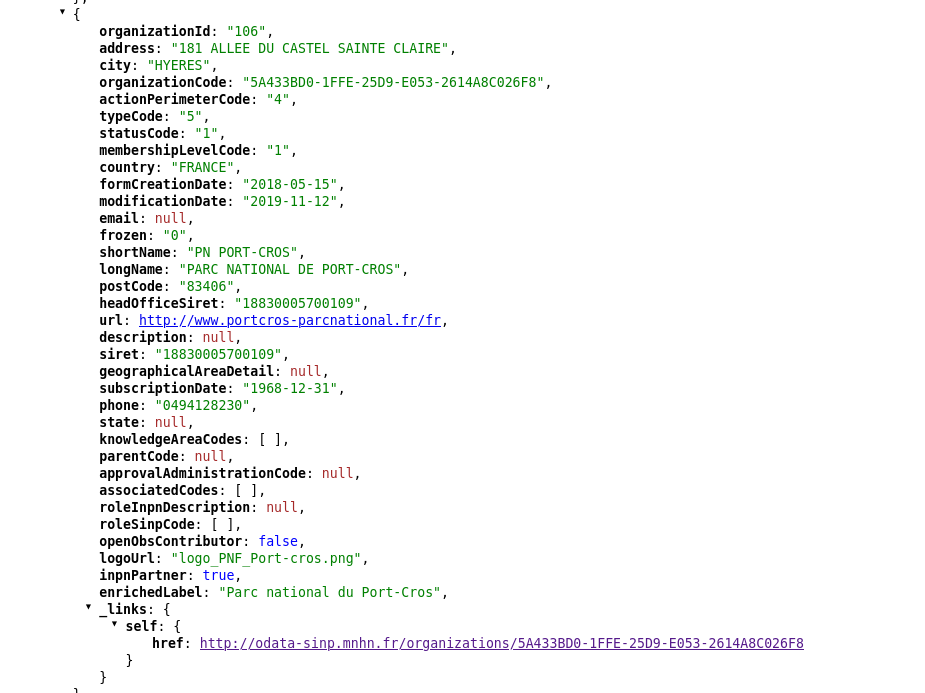
\includegraphics[width=0.8\textwidth]{includes/poc_inpn.png}
	\caption{Exemple d'entrée fournie par l'api INPN}
\end{figure}

Cette API couvre nos besoins en termes de tests, mais sera difficile à utiliser avec satisfaction pour le besoin exprimé ici. Je vois deux principaux obstacles :

\begin{itemize}
	\item La plupart des entrées texte sont tout en CAPITALES. Cela les rend difficilement utilisables dans les entrées de points de contact : c'est désagréable à lire tel quel, et délicat à convertir en minuscules. On peut certes les convertir en minuscules sauf la première lettre (mais quid des noms propres ?), ou chaque mot commence par une majuscule (mais ça ne présente pas toujours au mieux). Dans tous les cas, on perd les caractères accentués. Il aurait été préférable de stocker les entrées textes dans leur casse naturelle, il est toujours facile \textit{a posteriori} de les passer en majuscule quand le besoin se fait sentir.
	\item Le manque d'éléments de filtre. La base expose par défaut 7593 entrées, ça fait beaucoup. Il faudrait pouvoir filtrer les entrées et ne retenir que ce qui est vraiment pertinent. Le seul attribut qui me semble potentiellement utilisable est \texttt{inpnPartner}, ce qui réduit le nombre d'entrée à 104, mais je ne suis même pas sûr que ce soit pertinent.
\end{itemize}

\section*{Flux de traitement envisagés}
J'ai considéré deux principales chaines de traitement : 
\begin{enumerate}
	\item Collecter les entrées de l'API et pousser directement les entrées dans la base de données (court-circuiter \gn).
	\item Collecter les entrées de l'API, écrire les entrées sous forme de fichiers XML et les importer via \gn.
\end{enumerate}

\begin{figure}[hbtp]
	\centering
	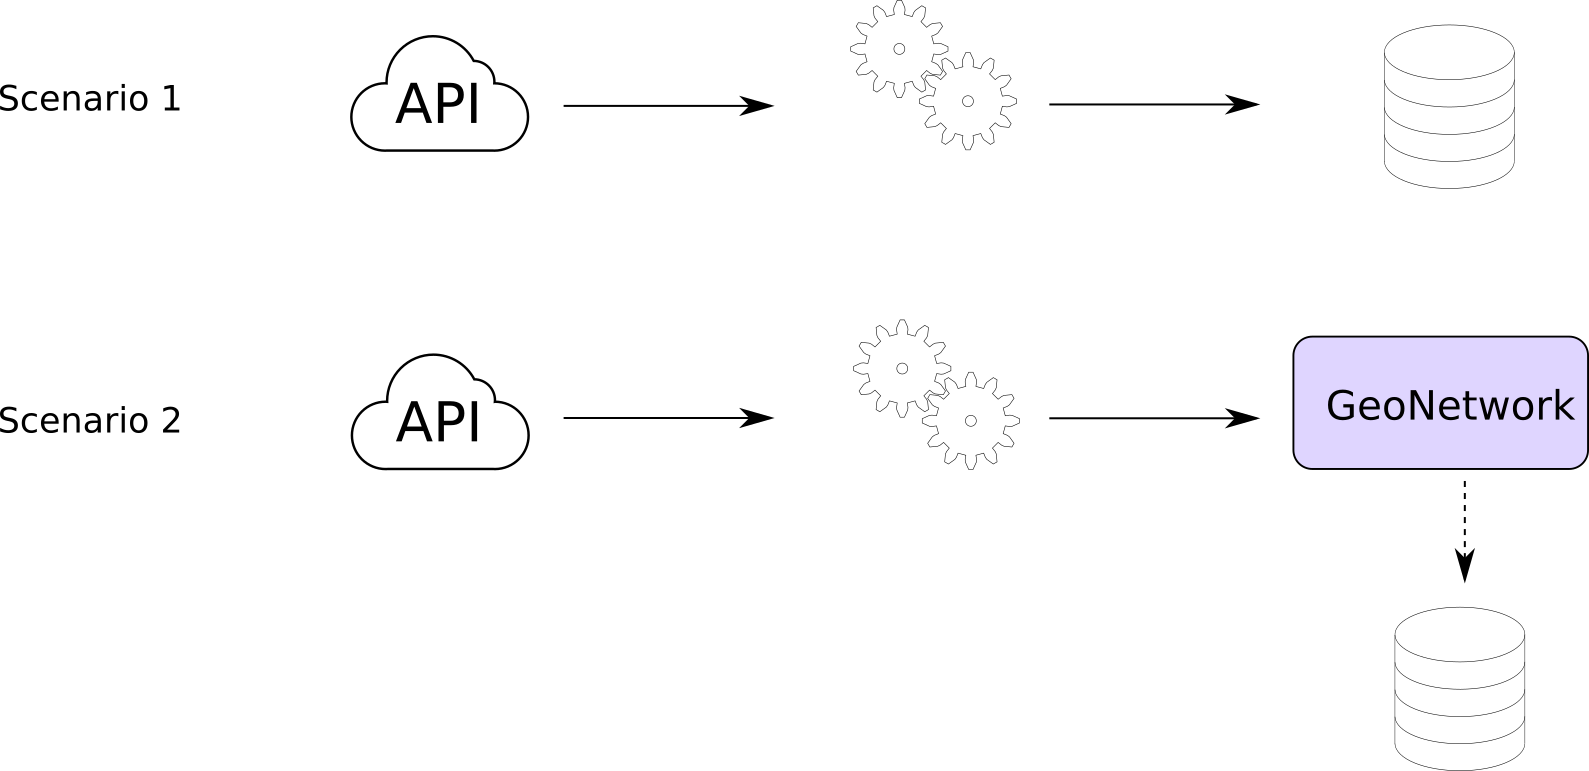
\includegraphics[width=0.8\textwidth]{includes/scenarii.png}
	\caption{Workflows envisagés}
\end{figure}

Le scenario 1 semble plus simple, mais est aussi plus fragile car la BD est gérée en principe par \gn et offre moins de possibilités que l'interface d'import de \gn.

Le scenario 2 est plus propre, on utilise le flux attendu, mais présente l'inconvénient de passer par authentification gérée par le CAS, un peu plus délicate à utiliser.

J'ai retenu le scenario 2. Le code écrit dans ce contexte pourra resservir sur d'autres besoins d'interactions avec l'API de \gn. 

Le flux de traitement se découpe en deux étapes :
\begin{enumerate}
	\item Collecter les entrées de l'API, écrire les entrées sous forme de fichier XML
	\item importer les fichiers XML dans \gn.
\end{enumerate}


\section*{API INPN -> XML}
C'est l'étape la plus simple : pas d'authentification, flux json, on est dans un cas standard.
Le code est sur \url{https://github.com/pi-geosolutions/contacts_sync/blob/main/src/contacts_api_to_xml.py}.

Le flux est le suivant : 

\begin{enumerate}
	\item On itère dans la pagination des données (gérée par l'API)
	\item Pour chaque page, pour chaque entrée dans la page, on récupère l'entrée sous forme de dict (clefs-valeur)
	\item et on fournit ce dict, à cahque fois, comme entrée sur un template Jinja2 : les valeurs fournies servent à alimenter un template de fichier XML
	\item et on sauvegarde le fichier XML ainsi généré, c'est notre point de contact sous forme de fragment XML conforme ISO 19139
\end{enumerate}

\section*{XML -> import dans \gn}
On a plusieurs façons de procéder:
\begin{itemize}
	\item Via l'interface graphique, fonction d'import : c'est la première que j'ai testé, pour m'assurer que les fichiers XML produits s'importaient correctement.
	\item Via l'API \gn, avec pour objectif de ne pas impliquer d'action manuelle. Plus compliqué, il faut gérer l'authentification via le CAS, de façon programmatique et manoeuvrer correctement l'API. C'est l'option que je retiens, bien sûr, puisque le but est de pouvoir automatiser le flux.
\end{itemize}
\vspace{0.5cm}

Dans les deux cas, on a plusieurs façons d'importer nos points de contact:
\begin{itemize}
	\item Un par un, on charge les fichiers XML. Bon pour tester, mauvais pour automatiser (long, nombreuses requêtes).
	\item Créer une archive MEF comme on fait pour les métadonnées, et import en groupe. L'inconvénient, c'est que je n'ai pas les spécifications d'une archive MEF pour ce type d'enregistrements.
	\item Il est aussi possible d'importer le contenu d'un dossier déposé sur le serveur, accessible par \gn via son système de fichiers. C'est un peu moins flexible, mais une option intéressante, pas trop compliquée à mettre en oeuvre dans notre configuration (composition docker, possibilité de monter les volumes partagés pour plusieurs conteneurs).
\end{itemize}

\vspace{0.5cm}
J'ai implémenté les solutions 1 et 3 (au choix via une option de commande). J'ai posé une question sur la mailing-list \gn pour avoir plus d'infos sur la piste 2 (archive MEF) qui pourrait être propre. Dans la pratique, je pense que la solution 3 est la meilleure pour nous.

\subsection*{Exemple de fichier importé dans \gn}
\lstinputlisting[basicstyle=\tiny,language=XML]{includes/biotope.xml}

\subsection*{Complications}
\subsubsection*{CAS}
L'authentification via le CAS m'a posé des soucis, car c'est un cas de figure modérément documenté.

Au final, la solution est assez étonnante de simplicité. Le prototype pour cette étape ne fait que quelques dizaines de lignes de code, aérées. La logique d'authentification fait une dizaine de lignes. On peut voir le résultat sur \url{https://github.com/pi-geosolutions/contacts_sync/blob/main/src/contacts_api_to_apiv2.py}.

\subsubsection*{API \gn}
Je n'ai pas trouvé l'API de \gn très facile à utiliser, malgré la mise à disposition d'une \href{https://sib1.dev.pigeosolutions.fr/geonetwork/doc/api/index.html#/}{interface swagger}, il m'a fallu un peu de temps pour m'y retrouver. Au final, l'endpoint d'import fonctionne bien, c'est en fait celui qui est utilisé par l'interface graphique, donc le fonctionnement est le même.

\subsection*{Script de la \textit{proof of concept}}
Le script "final" est \url{https://github.com/pi-geosolutions/contacts_sync/blob/main/src/contacts_api_to_apiv3.py}. Il est un peu plus long, mais c'est essentiellement la config du package \href{https://click.palletsprojects.com/en/8.1.x}{click} pour le rendre modulaire (options de script, possibilité de passer ces options via des variables d'environnement). 

Il reprend, dans son essence, les fonctions des deux autres scripts et propose au choix, soit de les lancer individuellement (pratique pour décortiquer et débugger) soir de chainer les deux traitements (option inpn-to-gn).

\subsubsection*{Mise en oeuvre en production}
Pour une mise en oeuvre en production, je préconise la méthode suivante : 

\begin{itemize}
	\item Création d'un dossier upload dans le volume geonetwork\_data
	\item Ajout d'un service dans la composition docker, avec une image docker contenant ce script (installation avec setuptools, idéalement)
	\begin{itemize}
		\item Le service resterait inactif mais tournerait en tâche de fond.
		\item Montage du dossier \lstinline{geonetwork_data/upload} comme volume
		\item Exécution du script via cron : 
		
		\begin{lstlisting}[language=bash]
		docker-compose exec contacts_sync contacts_api_to_api inpn-to-gn les_options_du_script
		\end{lstlisting}
		
	\end{itemize} 
\end{itemize}


\subsubsection*{Pistes d'améliorations}
Parmi les améliorations possibles : 

\begin{itemize}
	\item Permettre une mise à jour sélective des points de contact. l'API INPN fournissant un uuid pour chaque entrée, on peut détecter si une entrée dans l'annuaire de \gn vient du référentiel INPN. On peut donc à la prochaine mise à jour récupérer les deux sources, et mettre à jour le point de contact de façon sélective : n'actualiser que le nom et l'adresse par exemple, mais pas l'email ni le téléphone. Un traitement de ce genre sera nettement plus lent, puisqu'il faudra requêter l'API \gn pour récupérer chacune des entrées à concilier. Mais il n'y a pas de difficulté technique majeure.
	\item Finalisation du script. Il s'agit là d'une \textit{proof of concept}, mais il manque pas mal d'éléments pour en faire un script propre : 
	\begin{itemize}
		\item Robustifier le script : gestion des erreurs possibles (réseau, API, etc)
		\item Logging (pour l'instant on fait juste du printf)
		\item Rapportage / métriques pour le suivi du fonctionnement du script. On pourrait assez facilement écrire un fichier de métriques Prometheus (ou autre) pour suivi des métriques et alerting.
	\end{itemize} 
\end{itemize}


\section*{Conclusion}
Grâce à l'API de \gn, on voit qu'on peut envisager l'utilisation d'un référentiel de point de contact externe, avec une synchronisation régulière. On pourrait même envisager une mise à jour sélective de ces points de contacts, ce qui permettrait de récupérer des informations de base depuis le référentiel externe (nom de l'organisme, adresse) et de les compléter dans \gn (email, téléphone éventuellement, nom de personne).

L'essentiel du code écrit dans ce script est de l'enrobage (syntaxe click pour fonctions de CLI) mais la base de code pour faire cette synchronisation est pour l'instant très réduite. La mise à jour sélective augmenterait le volume de code, mais on resterait dans un cadre très raisonnable, assez facile à maintenir.

\end{document}